%
% Capítulo 1
%
\chapter{Introdução} \label{cap:intro}

Um sistema de \textit{Workflow} consiste numa plataforma que permite parametrizar, automatizar e monitorizar uma sequência de atividades que juntas compôem um processo de negócio.
Este tipo de sistema define o conjunto de regras para a execução das diferentes tarefas e determina os intervinentes em cada etapa desde a criação até à conclusão. Esta rigidez, promove a normalização de procedimentos e diminui a ocorrência de erros.
De forma complementar, um sistema de gestão documental permite armazenar, disponibilizar e controlar o acesso a documentos.
Estes sistemas têm o objetivo de garantir a integridade, confidencialidade e disponibilidade da informação.

No contexto da atividade da CAPT, estas duas componentes estão fortemente interligadas. Enquanto o sistema de \textit{workflow} coordena a execução das diferentes fases do processo de averiguação e a atribuição das respetivas responsabilidades, o sistema de gestão documental assegura que toda a documentação associada a cada processo, como fotografias, declarações, relatórios técnicos e restantes evidências, é armazenada, organizada e disponibilizada aos intervenientes autorizados.

Um processo de averiguação inicia-se com a receção, por parte da CAPT, de um pedido submetido por um dos seus clientes, habitualmente seguradoras, estes pedidos contêm informação preliminar relativa ao sinistro, nomeadamente a localização da ocorrência, os intervenientes envolvidos, a data deste, entre outros elementos relevantes para a abertura do processo de averiguação.

Atualmente, os pedidos são recebidos de forma não uniforme, o que introduz dificuldades operacionais no tratamento e acompanhamento dos processos, o que obriga os colaboradores da CAPT a recorrer a procedimentos pouco padronizados. A inexistência de uma plataforma centralizada limita ainda a capacidade da gestão em obter uma visão global da operação e em tomar decisões informadas, o que pode originar situações de distribuição desequilibrada de carga de trabalho e incumprimento de prazos.

Após a receção de um pedido de averiguação, é necessário proceder à sua análise e atribuição de um averiguador e de um supervisor. O averiguador desloca-se ao local da ocorrência, realiza as diligências necessárias, recolhendo evidências relevantes e elabora um relatório técnico que contém toda a informação apurada durante o processo de investigação. Posteriormente, esse relatório é submetido para validação pelo supervisor, responsável por garantir que o conteúdo produzido cumpre os padrões de qualidade e conformidade definidos pela CAPT antes da sua entrega ao cliente final.

Embora existam no mercado diversas plataformas de \textit{workflow} e gestão documental, estas são, na sua maioria, soluções de utilização genérica, concebidas para responder a um vasto conjunto de cenários organizacionais.
Consequentemente, disponibilizam funcionalidades que não são relevantes para a realidade operacional da CAPT e exigem frequentemente processos de configuração e adaptação complexos para acomodar fluxos de trabalho específicos.
Neste contexto, optou-se pelo desenvolvimento da plataforma IPW como uma solução personalizada, concebida de acordo com os procedimentos, intervenientes e regras de negócio da empresa.
Esta abordagem permite disponibilizar as funcionalidades necessárias, o que simplifica a utilização da plataforma pelos colaboradores e assegura um maior alinhamento com o processo de averiguação de sinistros adotado pela organização.

Para suportar esta organização operacional, foram definidos cinco perfis distintos de utilizador:

\begin{itemize}
  \item \textbf{Triador} — responsável pela receção dos pedidos de averiguação, criação de processos e pela sua atribuição aos averiguadores e supervisores;

  \item \textbf{Averiguador} — responsável pela realização das investigações no terreno e pela elaboração do respetivo relatório técnico;

  \item \textbf{Supervisor} — responsável pela validação dos relatórios técnicos produzidos pelos averiguadores de uma determinada área de especialização, como, por exemplo, sinistros automóveis ou acidentes de trabalho;

  \item \textbf{Gestor} — responsável pela validação final dos relatórios aprovados pelos supervisores, assegurando um segundo nível de controlo e supervisão sobre as diferentes áreas operacionais da organização;

  \item \textbf{Administrador} — responsável pela gestão da plataforma IPW, incluindo a criação de utilizadores, atribuição de perfis e gestão de permissões de acesso.

\end{itemize}

\begin{figure}[H]
  \begin{center}
    \resizebox{150mm}{!}{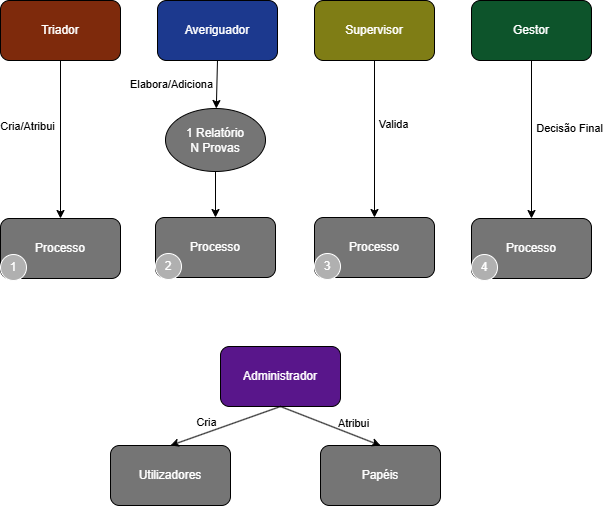
\includegraphics{./figures/cores_responsabilidade.drawio.png}}
  \end{center}
  \caption{Perfis de utilizadores na plataforma IPW.}\label{fig:responsabilidades}
\end{figure}

\newpage
\section{Objetivos}
O presente projeto tem como principal objetivo o desenvolvimento da plataforma \textit{Web}, \textit{IPW} \textit{(Insurance Portal Workflow)}, para suporte à gestão de processos de averiguação de sinistros da CAPT Consulting. A solução pretende melhorar a organização operacional da empresa, promovendo maior uniformização de procedimentos, rastreabilidade da informação e capacidade de monitorização da atividade.

De forma mais específica, definiram-se os seguintes objetivos:

\begin{itemize}
  \item Centralizar a informação relativa aos processos de averiguação numa única plataforma integrada;

  \item Estruturar o processo de atribuição e acompanhamento de averiguações entre os diferentes intervenientes da organização;

  \item Garantir o registo e rastreabilidade das interações realizadas ao longo do ciclo de vida de um processo;

  \item Disponibilizar mecanismos de gestão documental associados aos processos de averiguação;

  \item Fornecer indicadores operacionais e ferramentas de monitorização que suportem a supervisão e a tomada de decisão.

\end{itemize}


\section{Estado da Arte}
\label{sec:estado_da_arte}

No contexto empresarial existem várias plataformas destinadas à gestão documental, automação de processos e organização de fluxos de trabalho. Estas soluções procuram reduzir a dispersão de informação, normalizar procedimentos internos e permitir que diferentes utilizadores acompanhem tarefas, documentos e decisões ao longo do tempo.

Entre as soluções existentes no mercado, destacam-se plataformas como:
\begin{itemize}
  \item \textit{E-clic}~\cite{e-clic}: É uma plataforma empresarial de gestão documental e automação de \textit{workflows}, focada no controlo, organização e rastreabilidade de documentos e processos internos.
  \item \textit{DocuWare}~\cite{docuware}: Plataforma cloud de gestão documental e automação de \textit{workflows} empresariais, utilizada para digitalizar processos, arquivar documentos e controlar aprovações internas.
  \item \textit{Microsoft SharePoint}~\cite{sharepoint}: Plataforma colaborativa da \textit{Microsoft} focada na gestão de documentos, intranets corporativas e partilha de informação entre equipas. É amplamente utilizada em ambientes empresariais integrados com o ecossistema \textit{Microsoft 365}.
  \item \textit{SAP Build Process Automation}~\cite{sap-build-process-automation}: Solução empresarial da \textit{SAP} orientada para a automatização de processos, definição de fluxos de aprovação, integração com sistemas corporativos e monitorização de tarefas de negócio.
\end{itemize}

Apesar destas plataformas disponibilizarem funcionalidades relevantes, como armazenamento de documentos, controlo de acessos, colaboração, definição de fluxos de aprovação e integração com sistemas empresariais, tratam-se de soluções genéricas. A sua adoção num contexto específico, como a averiguação de sinistros, exigiria configuração, adaptação de processos e, em alguns casos, integração com sistemas externos para representar corretamente os papéis, estados e regras de negócio da organização.

A plataforma IPW distingue-se destas soluções por ter sido concebida especificamente para o contexto operacional da CAPT Consulting. Em vez de oferecer apenas mecanismos genéricos de gestão documental ou colaboração, o sistema modela diretamente o processo de averiguação de sinistros, incluindo papéis como triador, averiguador, supervisor, gestor e administrador, bem como estados próprios do ciclo de vida de um processo.

Nesta abordagem, a base de dados assume um papel central como fonte de verdade do \textit{workflow}, armazenando o estado atual de cada processo, o histórico de transições, os intervenientes responsáveis, os relatórios, as notas e os anexos associados. Esta decisão permite que o funcionamento do processo de averiguação seja representado diretamente no domínio da aplicação, em vez de depender apenas da configuração de uma plataforma genérica. Desta forma, a aplicação permite centralizar a informação de cada processo, controlar permissões de acordo com o papel ativo do utilizador e acompanhar a evolução do processo desde a sua criação até à aprovação final ou cancelamento.

Assim, embora existam soluções maduras no mercado para gestão documental e automação de \textit{workflows}, o desenvolvimento do IPW justifica-se pela necessidade de uma plataforma ajustada ao domínio específico da averiguação de sinistros, reduzindo a dependência de adaptações manuais e permitindo representar de forma mais direta o funcionamento interno da organização.

\section{Organização do documento}
O presente relatório encontra-se estruturado em quatro capítulos. No capítulo 1 procede-se ao enquadramento do problema, à apresentação dos objetivos do projeto e à contextualização da plataforma IPW.
No capítulo 2 descreve-se a solução proposta, incluindo a arquitetura do sistema, o modelo de dados e os principais aspetos de implementação das componentes \textit{backend} e \textit{frontend}.
No capítulo 3 apresenta-se a aplicação desenvolvida.
Finalmente, no capítulo 4 apresentam-se as conclusões do trabalho realizado e identificam-se as principais perspetivas de desenvolvimento futuro.
